\documentclass[11pt,a4paper]{article}

\usepackage[a4paper,margin=1in]{geometry}
\usepackage[T1]{fontenc}
\usepackage{lmodern}
\usepackage{booktabs}
\usepackage{amsmath}
\usepackage{pgfplots}
\usepgfplotslibrary{groupplots}
\pgfplotsset{compat=1.17}

\setlength{\parindent}{0pt}
\setlength{\parskip}{6pt}
\renewcommand{\arraystretch}{1.15}

\begin{document}

\begin{center}
{\Large Numerical Results}\\[0.5em]
{\normalsize 31 March 2026}
\end{center}

\section*{1 \quad Experimental Setting}

\[
S_0 = 100,\quad v_0 = 0.114,\quad v'_0 = 0.110,\quad r = 0,\quad T = 1,
\]
with
\[
\kappa_1 = 5.5,\quad \kappa_2 = 0.1,\quad \theta = 0.078,\quad \xi_1 = 2.689,\quad \xi_2 = 0.502,
\]
and
\[
\delta_1 = \delta_2 = 0.94,\quad \rho_{12} = -0.982,\quad \rho_{13} = -0.727,\quad \rho_{23} = 0.59.
\]

The Bermudan contract is sampled at \(12\) exercise dates. Five strike levels are considered:
\[
K \in \{70,80,90,100,110\},
\]
corresponding to deeper OTM through ITM puts.

All comparisons in this note use the fixed benchmark references generated with \(1200\) Euler steps. The reference direct prices are
\[
V^{\mathrm{ref}}_{110} = 16.645784,\quad V^{\mathrm{ref}}_{100} = 11.356823,\quad V^{\mathrm{ref}}_{90} = 7.402999,
\]
\[
V^{\mathrm{ref}}_{80} = 4.596899,\quad V^{\mathrm{ref}}_{70} = 2.699339.
\]

For any direct price estimate \(V\) and reference value \(V^{\mathrm{ref}}\), the direct relative error is defined by
\[
\varepsilon_{\mathrm{dir}} = \frac{|V - V^{\mathrm{ref}}|}{|V^{\mathrm{ref}}|}.
\]

The \(95\%\) confidence interval is reported as
\[
V \pm 1.96\,\mathrm{SE},
\]
and the confidence-interval width is therefore \(2 \times 1.96 \times \mathrm{SE}\).

The objective is to compare plain LSMC with the Hybrid LSMC--PDE method under \emph{matched path budgets}. Two matched-path regimes are examined:
\begin{itemize}
\item \(60{,}000\) direct paths for both methods;
\item \(20{,}000\) direct paths for both methods.
\end{itemize}

The Euler step counts are \(24,48,72,96\). The hybrid numerical setting is kept fixed at \(301\) asset grid points, asset range factors \(0.30\) and \(3.50\), and volatility truncation quantile \(0.999\).

\section*{2 \quad Matched 60,000-Path Comparison}

Table~1 shows the Euler steps at which the Hybrid LSMC--PDE method achieves a smaller direct error than plain LSMC when both methods use \(60{,}000\) direct paths.

\begin{table}[h!]
\centering
\caption{Hybrid win counts under the matched 60,000-path comparison.}
\begin{tabular}{lc}
\toprule
Scenario & Hybrid better at steps \\
\midrule
ITM put & 48, 72, 96 \\
ATM & 48, 72 \\
OTM put & 48, 72 \\
K = 80 put & 48, 72, 96 \\
K = 70 put & 24, 48, 72, 96 \\
\bottomrule
\end{tabular}
\end{table}

The main favorable region is the middle of the step grid, especially \(48\) to \(72\) steps.

\begin{figure}[p]
\centering
\begin{tikzpicture}
\begin{groupplot}[
group style={group size=2 by 3, horizontal sep=1.8cm, vertical sep=1.8cm},
width=0.43\textwidth,
height=0.24\textheight,
xmin=22, xmax=98,
ymin=0, ymax=8.5,
xtick={24,48,72,96},
ylabel={Direct relative error (\%)},
xlabel={Euler steps},
grid=major,
grid style={draw=gray!20},
axis line style={draw=black!60},
tick style={draw=black!60},
title style={font=\small},
label style={font=\small},
tick label style={font=\small},
legend style={font=\small, draw=none, fill=none},
]
\nextgroupplot[title={ITM put}]
\addplot[blue, thick, mark=*] coordinates {(24,1.926) (48,0.501) (72,0.837) (96,0.360)};
\addplot[orange!85!black, thick, mark=square*] coordinates {(24,1.966) (48,0.439) (72,0.048) (96,0.081)};
\legend{LSMC, Hybrid LSMC--PDE}

\nextgroupplot[title={ATM}]
\addplot[blue, thick, mark=*] coordinates {(24,2.415) (48,1.232) (72,1.227) (96,0.310)};
\addplot[orange!85!black, thick, mark=square*] coordinates {(24,2.590) (48,0.302) (72,0.216) (96,0.412)};

\nextgroupplot[title={OTM put}]
\addplot[blue, thick, mark=*] coordinates {(24,3.523) (48,1.769) (72,1.363) (96,0.112)};
\addplot[orange!85!black, thick, mark=square*] coordinates {(24,3.731) (48,0.526) (72,0.139) (96,0.449)};

\nextgroupplot[title={K = 80 put}]
\addplot[blue, thick, mark=*] coordinates {(24,5.336) (48,2.870) (72,1.429) (96,0.531)};
\addplot[orange!85!black, thick, mark=square*] coordinates {(24,5.385) (48,1.128) (72,0.287) (96,0.167)};

\nextgroupplot[title={K = 70 put}]
\addplot[blue, thick, mark=*] coordinates {(24,7.760) (48,3.791) (72,2.482) (96,0.437)};
\addplot[orange!85!black, thick, mark=square*] coordinates {(24,7.297) (48,1.906) (72,0.847) (96,0.264)};

\nextgroupplot[title={Reading note}, axis lines=none, xtick=\empty, ytick=\empty]
\node[align=left, anchor=west, font=\small] at (rel axis cs:0.05,0.82) {At 60,000 paths, the hybrid method is strongest in the};
\node[align=left, anchor=west, font=\small] at (rel axis cs:0.05,0.66) {middle of the grid, especially at 48 and 72 steps.};
\node[align=left, anchor=west, font=\small] at (rel axis cs:0.05,0.50) {Some edge cases at 24 and 96 steps still favor LSMC.};
\end{groupplot}
\end{tikzpicture}
\caption{Direct relative error under the matched 60,000-path comparison.}
\end{figure}

\begin{figure}[p]
\centering
\begin{tikzpicture}
\begin{groupplot}[
group style={group size=2 by 3, horizontal sep=1.8cm, vertical sep=1.8cm},
width=0.43\textwidth,
height=0.24\textheight,
xmin=22, xmax=98,
ymin=0, ymax=0.34,
xtick={24,48,72,96},
ylabel={95\% CI width},
xlabel={Euler steps},
grid=major,
grid style={draw=gray!20},
axis line style={draw=black!60},
tick style={draw=black!60},
title style={font=\small},
label style={font=\small},
tick label style={font=\small},
legend style={font=\small, draw=none, fill=none},
]
\nextgroupplot[title={ITM put}]
\addplot[blue, thick, mark=*] coordinates {(24,0.310742) (48,0.311805) (72,0.314858) (96,0.304737)};
\addplot[orange!85!black, thick, mark=square*] coordinates {(24,0.101642) (48,0.102497) (72,0.102736) (96,0.102563)};
\legend{LSMC, Hybrid LSMC--PDE}

\nextgroupplot[title={ATM}]
\addplot[blue, thick, mark=*] coordinates {(24,0.270574) (48,0.272726) (72,0.271095) (96,0.263530)};
\addplot[orange!85!black, thick, mark=square*] coordinates {(24,0.079830) (48,0.080645) (72,0.081018) (96,0.080879)};

\nextgroupplot[title={OTM put}]
\addplot[blue, thick, mark=*] coordinates {(24,0.228650) (48,0.224475) (72,0.222460) (96,0.219512)};
\addplot[orange!85!black, thick, mark=square*] coordinates {(24,0.058877) (48,0.059512) (72,0.059951) (96,0.059815)};

\nextgroupplot[title={K = 80 put}]
\addplot[blue, thick, mark=*] coordinates {(24,0.183519) (48,0.178466) (72,0.176102) (96,0.174954)};
\addplot[orange!85!black, thick, mark=square*] coordinates {(24,0.040868) (48,0.041240) (72,0.041668) (96,0.041516)};

\nextgroupplot[title={K = 70 put}]
\addplot[blue, thick, mark=*] coordinates {(24,0.140250) (48,0.134440) (72,0.134585) (96,0.132335)};
\addplot[orange!85!black, thick, mark=square*] coordinates {(24,0.026589) (48,0.026738) (72,0.027079) (96,0.026897)};

\nextgroupplot[title={Reading note}, axis lines=none, xtick=\empty, ytick=\empty]
\node[align=left, anchor=west, font=\small] at (rel axis cs:0.05,0.82) {The confidence intervals are substantially narrower};
\node[align=left, anchor=west, font=\small] at (rel axis cs:0.05,0.66) {for the hybrid method at the same 60,000-path budget.};
\node[align=left, anchor=west, font=\small] at (rel axis cs:0.05,0.50) {This is one of the strongest stable findings of the study.};
\end{groupplot}
\end{tikzpicture}
\caption{95\% confidence-interval width under the matched 60,000-path comparison.}
\end{figure}

Table~2 reports representative results at \(72\) steps, including direct prices, \(95\%\) confidence intervals, and runtime.

\begin{table}[p]
\centering
\caption{Representative \(72\)-step values under the matched 60,000-path comparison.}
\begin{tabular}{lcccccc}
\toprule
& \multicolumn{3}{c}{LSMC} & \multicolumn{3}{c}{Hybrid LSMC--PDE} \\
\cmidrule(lr){2-4}\cmidrule(lr){5-7}
Scenario & Direct price & 95\% CI & Runtime & Direct price & 95\% CI & Runtime \\
\midrule
ITM put & 16.785116 & [16.627687, 16.942545] & 1.18 s & 16.653809 & [16.602442, 16.705177] & 238.75 s \\
ATM & 11.496193 & [11.360645, 11.631741] & 1.25 s & 11.332296 & [11.291787, 11.372805] & 241.84 s \\
OTM put & 7.503911 & [7.392681, 7.615141] & 1.16 s & 7.392732 & [7.362757, 7.422707] & 240.15 s \\
K = 80 put & 4.662578 & [4.574527, 4.750629] & 1.17 s & 4.610083 & [4.589249, 4.630917] & 230.58 s \\
K = 70 put & 2.766338 & [2.699045, 2.833631] & 1.21 s & 2.722197 & [2.708657, 2.735737] & 233.90 s \\
\bottomrule
\end{tabular}
\end{table}

\section*{3 \quad Matched 20,000-Path Comparison}

The matched path budget was then reduced from \(60{,}000\) to \(20{,}000\) for both methods.

\begin{table}[h!]
\centering
\caption{Hybrid win counts under the matched 20,000-path comparison.}
\begin{tabular}{lc}
\toprule
Scenario & Hybrid better at steps \\
\midrule
ITM put & 24, 48, 72, 96 \\
ATM & 24, 48, 72, 96 \\
OTM put & 24, 48, 72, 96 \\
K = 80 put & 24, 48, 72, 96 \\
K = 70 put & 24, 48, 72 \\
\bottomrule
\end{tabular}
\end{table}

Reducing the path budget strengthens the favorable direct-error result. The benchmark LSMC method deteriorates faster than the hybrid method, so the hybrid advantage becomes broader across the step grid.

\begin{figure}[p]
\centering
\begin{tikzpicture}
\begin{groupplot}[
group style={group size=2 by 3, horizontal sep=1.8cm, vertical sep=1.8cm},
width=0.43\textwidth,
height=0.24\textheight,
xmin=22, xmax=98,
ymin=0, ymax=9.5,
xtick={24,48,72,96},
ylabel={Direct relative error (\%)},
xlabel={Euler steps},
grid=major,
grid style={draw=gray!20},
axis line style={draw=black!60},
tick style={draw=black!60},
title style={font=\small},
label style={font=\small},
tick label style={font=\small},
legend style={font=\small, draw=none, fill=none},
]
\nextgroupplot[title={ITM put}]
\addplot[blue, thick, mark=*] coordinates {(24,2.570) (48,1.221) (72,0.773) (96,0.561)};
\addplot[orange!85!black, thick, mark=square*] coordinates {(24,1.468) (48,0.228) (72,0.163) (96,0.407)};
\legend{LSMC, Hybrid LSMC--PDE}

\nextgroupplot[title={ATM}]
\addplot[blue, thick, mark=*] coordinates {(24,4.025) (48,1.336) (72,0.948) (96,1.694)};
\addplot[orange!85!black, thick, mark=square*] coordinates {(24,2.001) (48,0.052) (72,0.475) (96,0.172)};

\nextgroupplot[title={OTM put}]
\addplot[blue, thick, mark=*] coordinates {(24,5.623) (48,2.173) (72,1.788) (96,1.994)};
\addplot[orange!85!black, thick, mark=square*] coordinates {(24,3.118) (48,0.248) (72,0.418) (96,0.253)};

\nextgroupplot[title={K = 80 put}]
\addplot[blue, thick, mark=*] coordinates {(24,7.445) (48,3.193) (72,1.645) (96,1.742)};
\addplot[orange!85!black, thick, mark=square*] coordinates {(24,4.810) (48,0.832) (72,0.012) (96,0.668)};

\nextgroupplot[title={K = 70 put}]
\addplot[blue, thick, mark=*] coordinates {(24,8.911) (48,3.890) (72,1.476) (96,0.748)};
\addplot[orange!85!black, thick, mark=square*] coordinates {(24,6.757) (48,1.589) (72,0.560) (96,1.186)};

\nextgroupplot[title={Reading note}, axis lines=none, xtick=\empty, ytick=\empty]
\node[align=left, anchor=west, font=\small] at (rel axis cs:0.05,0.82) {At 20,000 paths the benchmark method deteriorates faster,};
\node[align=left, anchor=west, font=\small] at (rel axis cs:0.05,0.66) {so the hybrid advantage becomes much more visible.};
\node[align=left, anchor=west, font=\small] at (rel axis cs:0.05,0.50) {Only the K = 70 case at 96 steps still favors LSMC.};
\end{groupplot}
\end{tikzpicture}
\caption{Direct relative error under the matched 20,000-path comparison.}
\end{figure}

\begin{figure}[p]
\centering
\begin{tikzpicture}
\begin{groupplot}[
group style={group size=2 by 3, horizontal sep=1.8cm, vertical sep=1.8cm},
width=0.43\textwidth,
height=0.24\textheight,
xmin=22, xmax=98,
ymin=0, ymax=0.56,
xtick={24,48,72,96},
ylabel={95\% CI width},
xlabel={Euler steps},
grid=major,
grid style={draw=gray!20},
axis line style={draw=black!60},
tick style={draw=black!60},
title style={font=\small},
label style={font=\small},
tick label style={font=\small},
legend style={font=\small, draw=none, fill=none},
]
\nextgroupplot[title={ITM put}]
\addplot[blue, thick, mark=*] coordinates {(24,0.527546) (48,0.531415) (72,0.528510) (96,0.535503)};
\addplot[orange!85!black, thick, mark=square*] coordinates {(24,0.175654) (48,0.178423) (72,0.177942) (96,0.178438)};
\legend{LSMC, Hybrid LSMC--PDE}

\nextgroupplot[title={ATM}]
\addplot[blue, thick, mark=*] coordinates {(24,0.464500) (48,0.467617) (72,0.460326) (96,0.467433)};
\addplot[orange!85!black, thick, mark=square*] coordinates {(24,0.138103) (48,0.140771) (72,0.140765) (96,0.141113)};

\nextgroupplot[title={OTM put}]
\addplot[blue, thick, mark=*] coordinates {(24,0.395669) (48,0.388072) (72,0.386771) (96,0.385951)};
\addplot[orange!85!black, thick, mark=square*] coordinates {(24,0.102055) (48,0.104195) (72,0.104563) (96,0.104748)};

\nextgroupplot[title={K = 80 put}]
\addplot[blue, thick, mark=*] coordinates {(24,0.316003) (48,0.305423) (72,0.300813) (96,0.299696)};
\addplot[orange!85!black, thick, mark=square*] coordinates {(24,0.071023) (48,0.072507) (72,0.073089) (96,0.073010)};

\nextgroupplot[title={K = 70 put}]
\addplot[blue, thick, mark=*] coordinates {(24,0.239794) (48,0.232088) (72,0.226584) (96,0.227627)};
\addplot[orange!85!black, thick, mark=square*] coordinates {(24,0.046341) (48,0.047312) (72,0.047847) (96,0.047525)};

\nextgroupplot[title={Reading note}, axis lines=none, xtick=\empty, ytick=\empty]
\node[align=left, anchor=west, font=\small] at (rel axis cs:0.05,0.82) {The confidence-interval advantage of the hybrid method};
\node[align=left, anchor=west, font=\small] at (rel axis cs:0.05,0.66) {remains very strong after the path budget is reduced to 20,000.};
\node[align=left, anchor=west, font=\small] at (rel axis cs:0.05,0.50) {This helps explain why its direct-error ranking improves.};
\end{groupplot}
\end{tikzpicture}
\caption{95\% confidence-interval width under the matched 20,000-path comparison.}
\end{figure}

Table~4 reports representative \(72\)-step values for the \(20{,}000\)-path comparison.

\begin{table}[p]
\centering
\caption{Representative \(72\)-step values under the matched 20,000-path comparison.}
\begin{tabular}{lcccccc}
\toprule
& \multicolumn{3}{c}{LSMC} & \multicolumn{3}{c}{Hybrid LSMC--PDE} \\
\cmidrule(lr){2-4}\cmidrule(lr){5-7}
Scenario & Direct price & 95\% CI & Runtime & Direct price & 95\% CI & Runtime \\
\midrule
ITM put & 16.774434 & [16.510179, 17.038689] & 0.43 s & 16.618575 & [16.529605, 16.707546] & 76.22 s \\
ATM & 11.464532 & [11.234369, 11.694695] & 0.46 s & 11.302836 & [11.232454, 11.373219] & 78.05 s \\
OTM put & 7.535388 & [7.342003, 7.728773] & 0.50 s & 7.372034 & [7.319752, 7.424315] & 78.74 s \\
K = 80 put & 4.672537 & [4.522131, 4.822943] & 0.49 s & 4.597431 & [4.560886, 4.633975] & 78.68 s \\
K = 70 put & 2.739173 & [2.625881, 2.852465] & 0.50 s & 2.714444 & [2.690521, 2.738368] & 78.67 s \\
\bottomrule
\end{tabular}
\end{table}

\section*{4 \quad Conclusions}

\begin{itemize}
\item Under the matched \(60{,}000\)-path comparison, the Hybrid LSMC--PDE method is most favorable in the middle of the Euler grid, especially at \(48\) and \(72\) steps. Some edge cases at \(24\) and \(96\) steps still favor plain LSMC.
\item Under the matched \(20{,}000\)-path comparison, the favorable hybrid result becomes stronger. The benchmark LSMC method deteriorates faster, and the hybrid method becomes more accurate in almost all tested cases.
\item In both matched-path regimes, the hybrid method has much smaller standard errors and much narrower confidence intervals across the full strike range. This is one of the clearest robust findings of the study.
\item The main cost of the hybrid method remains runtime. Plain LSMC is substantially faster in both cases, even when it is less accurate and less stable at equal path budgets.
\end{itemize}

Taken together, the two matched-path studies show a consistent pattern. When the comparison is made on a fair equal-path basis, the Hybrid LSMC--PDE method performs particularly well at moderate Euler resolutions. Moreover, when the path budget is tightened, the hybrid advantage becomes even more visible because its confidence intervals remain much narrower than those of plain LSMC.

\end{document}
